%!TEX program = xelatex
%!TEX root = ../all.tex
\chapter{Probability recall}

\section*{Discrete Random Variables}

In order to reason rigorously about uncertainty, we introduce the notion of a discrete \alert{random variable} $X$. Conceptually, a random variable is not a variable in the algebraic sense, but rather a formal device that represents the outcome of a stochastic experiment or process. The possible outcomes that $X$ can take belong to a finite or countably infinite set, which we denote by $\mathcal{X}$. Each realization of the experiment corresponds to exactly one element of this set.

The probabilistic behavior of $X$ is completely characterized by its \alert{probability mass function} (pmf). The pmf assigns to each possible outcome $x\in\mathcal{X}$ a number $p(X=x)$ that quantifies how likely it is for the random variable to take that value. For simplicity of notation, and following common practice, we will often denote the event $X=x$ simply by $x$, writing $p(x)$ instead of $p(X=x)$ whenever no ambiguity arises.

\subsubsection*{Fundamental Properties}

Not every function from $\mathcal{X}$ to $\mathbb{R}$ can be interpreted as a probability mass function. In order to be meaningful, a pmf must satisfy two basic axioms that encode our intuitive understanding of probability. First, probabilities must be non-negative and bounded above by one: an event cannot occur with negative likelihood, nor can it be more than certain. Formally,
\begin{myequation}
0 \leq p(x) \leq 1 \quad \text{for all } x \in \mathcal{X}.
\end{myequation}
Second, since the random variable must assume exactly one value in its domain whenever the experiment is performed, the probabilities of all mutually exclusive outcomes must sum to one. This is the normalization condition,
\begin{myequation}
\sum_{x \in \mathcal{X}} p(x) = 1.
\end{myequation}
Together, these two properties ensure that the pmf provides a complete and consistent description of uncertainty over $\mathcal{X}$. Any function satisfying them qualifies as a valid probability distribution.

\subsubsection*{Joint and Conditional Probabilities}

In realistic settings, we rarely deal with a single random variable in isolation. Instead, we are often interested in the relationships between multiple variables. Given two events $x$ and $y$ corresponding to two (possibly different) random variables, we distinguish between joint and conditional probabilities.

The \alert{joint probability} $p(x,y)$, also written as $p(x \wedge y)$, represents the probability that both events occur simultaneously. It captures the full interaction between $x$ and $y$, describing how they behave together rather than individually. The \alert{conditional probability} $p(x|y)$, on the other hand, quantifies the probability that $x$ occurs under the assumption that $y$ has already occurred. Conceptually, it describes how our belief about $x$ should be updated once we have observed $y$.

These two notions are linked by the \alert{product rule}, which formalizes the intuitive idea that the probability of two events occurring together can be decomposed into a sequential structure:
\begin{myequation}
p(x,y) = p(x|y)p(y) = p(y|x)p(x).
\end{myequation}
The probabilities $p(x)$ and $p(y)$ appearing on their own are called \alert{marginal probabilities}, as they describe the behavior of a single variable irrespective of the values taken by other variables. The symmetry of the joint probability---meaning that $p(x,y)=p(y,x)$---together with the product rule gives rise to the two decompositions shown above, which will later lead directly to Bayes' rule.

The product rule extends naturally to more than two variables. For a collection of $n$ random variables $x_1,\ldots,x_n$, it yields the \alert{chain rule} of probability, which allows a high-dimensional joint distribution to be factorized into a product of conditional distributions:
\begin{myalign}
p(x_1,\ldots,x_n)
&= p(x_2,\ldots,x_n|x_1)p(x_1) \\
&= p(x_3,\ldots,x_n|x_1,x_2)p(x_2|x_1)p(x_1) \\
&\;\;\vdots \\
&= p(x_n|x_1,\ldots,x_{n-1})p(x_{n-1}|x_1,\ldots,x_{n-2})\cdots p(x_2|x_1)p(x_1).
\end{myalign}
This factorization plays a central role in probabilistic modeling, as it provides a systematic way to construct complex joint distributions from simpler conditional components. It also forms the mathematical foundation for graphical models, where conditional independencies allow certain factors in this chain to simplify.

\subsubsection*{Union of Events}

Another common operation involves computing the probability that at least one of two events occurs. This corresponds to the probability of the union $x \vee y$, and the correct formula is given by the inclusion--exclusion principle:
\begin{myequation}
p(x \vee y) = p(x) + p(y) - p(x,y).
\end{myequation}
The subtraction of the joint probability is necessary to avoid counting the overlap between $x$ and $y$ twice: if both events occur simultaneously, that outcome would otherwise be counted once in $p(x)$ and once again in $p(y)$. In the special case where the two events are \alert{mutually exclusive}---meaning they cannot occur simultaneously, so $p(x,y)=0$---the expression simplifies to
\begin{myequation}
p(x \vee y) = p(x) + p(y).
\end{myequation}
This situation often arises when $x$ and $y$ represent distinct outcomes of the same random variable, which by definition cannot take two values at once.

\subsubsection*{The Sum Rule and Marginalization}

While the product rule allows us to build joint probabilities, the \alert{sum rule} allows us to reduce them by eliminating variables we are not interested in. Suppose we know the joint distribution $p(x,y)$ but wish to compute the marginal distribution of $x$ alone. This is done by summing over all possible values of $y$:
\begin{myequation}
p(x) = \sum_{y \in \mathcal{Y}} p(x,y)
      = \sum_{y \in \mathcal{Y}} p(x|y)p(y).
\end{myequation}
This operation is known as \alert{marginalization}. Conceptually, it corresponds to averaging over all possible states of $Y$, thereby collapsing the joint distribution onto the subspace associated with $X$ alone. The second form of the expression, obtained by applying the product rule to $p(x,y)$, is sometimes called the \emph{law of total probability}: it expresses the unconditional probability of $x$ as a weighted average of the conditional probabilities $p(x|y)$, weighted by how probable each conditioning event $y$ is.

\subsubsection*{Bayes' Rule}

By combining the product rule with the sum rule, we arrive at one of the most important identities in probability theory: \alert{Bayes' rule}. Starting from the symmetry of the joint distribution,
\begin{myalign}
p(x,y) &= p(x|y)p(y), \\
p(x,y) &= p(y|x)p(x),
\end{myalign}
and equating the right-hand sides, we obtain
\begin{myequation}
p(x|y) = \frac{p(y|x)p(x)}{p(y)}.
\end{myequation}
Using the sum rule to express the marginal $p(y)$ explicitly, this can be written as
\begin{myequation}
p(x|y) = \frac{p(y|x)p(x)}{\sum_{x \in \mathcal{X}} p(y|x)p(x)}.
\end{myequation}

Bayes' rule provides a formal mechanism for learning from data. The term $p(x)$ is the \alert{prior}, representing our belief about $x$ before observing $y$. The likelihood $p(y|x)$ measures how compatible the observation is with the hypothesis $x$. The result, $p(x|y)$, is the \alert{posterior}---an updated belief that incorporates the new evidence. The denominator $p(y)$, often called the \alert{evidence} or marginal likelihood, ensures proper normalization: it represents the total probability of observing $y$ under all possible states of $x$, and plays a crucial role in model comparison. Throughout this text, Bayes' rule will return repeatedly as the backbone of Bayesian inference.

\subsection*{Independence}

The concept of independence formalizes the idea that some variables do not influence each other. Two random variables $X$ and $Y$ are said to be \alert{independent}, denoted $\ind{X}{Y}$, if their joint distribution factorizes into the product of their marginals:
\begin{myequation}
p(x,y) = p(x)p(y).
\end{myequation}
Intuitively, this means that observing one variable provides no information about the other. This intuition becomes explicit when we apply the product rule: if $X$ and $Y$ are independent, then $p(x|y) = p(x)$ and $p(y|x) = p(y)$, confirming that conditioning on one variable leaves the other unchanged. Independence is a very strong structural assumption, but when it holds it leads to enormous simplifications---joint distributions factorize, expectations of products equal products of expectations, and variances of sums equal sums of variances.

\subsubsection*{Conditional Independence}

Independence can also arise only after conditioning on a third variable. Two variables $X$ and $Y$ are said to be \alert{conditionally independent} given a third variable $Z$, written $\cind{X}{Y}{Z}$, if
\begin{myequation}
p(x,y|z) = p(x|z)p(y|z).
\end{myequation}
This notion is more subtle than unconditional independence. Variables that are dependent in general may become independent once additional information is taken into account. Conversely, variables that are marginally independent may become dependent when conditioning on a third variable.

A classic illustration is the \alert{common cause} structure. Consider shoe size $X$ and reading ability $Y$ in elementary school children, with age $Z$ as a mediating variable. Marginally, shoe size and reading ability are correlated, because both tend to increase with age:
\begin{myequation}
p(x,y) \neq p(x)p(y).
\end{myequation}
However, once age is known, shoe size provides no additional information about reading ability:
\begin{myequation}
p(x,y|z) = p(x|z)p(y|z).
\end{myequation}
In this case, the apparent dependence between $X$ and $Y$ is entirely explained by their shared dependence on $Z$. This structure, often depicted as $X \leftarrow Z \rightarrow Y$, is one of the fundamental building blocks of probabilistic graphical models and causal reasoning. Understanding which dependencies are real and which are induced by a common cause is essential in data analysis, as it determines whether an observed correlation has a meaningful causal interpretation.


\section*{Continuous Random Variables}

While discrete random variables are appropriate when the set of possible outcomes is finite or countable, many phenomena encountered in practice are more naturally described by a continuum of values. Examples include physical quantities such as time, temperature, position, or voltage. A \alert{continuous random variable} $X$ takes values in an uncountable set $\mathcal{X}$, typically the real line $\mathbb{R}$ or an interval of it.

A fundamental conceptual difference with respect to the discrete case is that, for a continuous random variable, the probability of observing any \emph{exact} value is zero:
\begin{myequation}
p(X=x)=0 \quad \text{for every } x \in \mathcal{X}.
\end{myequation}
This does not mean the event $X=x$ is impossible in a deterministic sense, but rather that probability mass is spread continuously over infinitely many points, so no single point carries a positive share. As a consequence, probabilities are no longer assigned to individual points, but to intervals and more general measurable sets.

To describe the distribution of $X$, we therefore introduce the \alert{cumulative distribution function} (cdf), defined as
\begin{myequation}
F(x)=p(X\leq x).
\end{myequation}
The cdf accumulates probability from $-\infty$ up to $x$ and provides a complete characterization of the distribution. Once $F(x)$ is known, the probability that $X$ falls in any interval $(a,b]$ is obtained by subtraction:
\begin{myequation}
p(a < X \leq b) = F(b) - F(a).
\end{myequation}
This mirrors the discrete case, where probabilities of sets are obtained by summing probabilities of individual outcomes; here summation over a continuum is replaced by accumulation through $F$.

\subsubsection*{The Probability Density Function}

Although the cdf is conceptually fundamental, it is often more convenient to work with a function that describes how probability is locally distributed along the real line. This leads to the \alert{probability density function} (pdf), defined---whenever the cdf is differentiable---as its derivative:
\begin{myequation}
f(x)=\frac{dF(x)}{dx}.
\end{myequation}
The pdf does not represent a probability by itself; instead, it represents a \emph{density} of probability. Its interpretation becomes clear when considering a small interval of width $dx$ around $x$: the probability that $X$ falls in this interval is approximately $f(x)\,dx$, meaning
\begin{myequation}
p(x < X \leq x+dx) \approx f(x)\,dx.
\end{myequation}
Larger values of $f(x)$ therefore indicate regions where the random variable is more likely to be found. To compute the probability over a finite interval $[a,b]$, these infinitesimal contributions are accumulated through integration:
\begin{myequation}
p(a < X \leq b) = \int_a^b f(x)\,dx.
\end{myequation}
Consistency with the axioms of probability requires two conditions: $f(x)\ge 0$ for all $x$, ensuring probabilities are non-negative, and
\begin{myequation}
\int_{-\infty}^{\infty} f(x)\,dx = 1,
\end{myequation}
ensuring total probability is one. Note that $f(x)$ itself can exceed one: it is a density, not a probability, and its value at a point is only meaningful relative to the scale of the surrounding region.

\subsection*{Extension to Multiple Variables}

The core rules of probability theory extend seamlessly from discrete to continuous random variables. The conceptual structure remains the same; the only technical change is that sums over discrete states are replaced by integrals over continuous domains. Consider two continuous random variables $X$ and $Y$ with joint probability density $f(x,y)$. Often we are interested only in the distribution of one variable, regardless of the value taken by the other. The continuous analogue of the sum rule allows us to recover the marginal density of $X$ by integrating out $Y$:
\begin{myequation}
f(x)=\int_{\mathcal{Y}} f(x,y)\,dy.
\end{myequation}
Using the product rule for densities, this can also be written as
\begin{myequation}
f(x)=\int_{\mathcal{Y}} f(x|y)f(y)\,dy.
\end{myequation}
This expression highlights an important interpretation: the marginal density of $X$ is a weighted average of the conditional densities $f(x|y)$, where the weights are given by how probable each value of $y$ is. The joint and marginal densities naturally define the \alert{conditional density} of $X$ given $Y$ as
\begin{myequation}
f(x|y)=\frac{f(x,y)}{f(y)},
\end{myequation}
which describes how the distribution of $X$ changes once the value of $Y$ is known. If learning $Y=y$ does not affect our uncertainty about $X$, then the two variables are \alert{independent}, their joint density factorizes as $f(x,y)=f(x)f(y)$, and the conditional density reduces to the marginal, $f(x|y)=f(x)$.

\subsection*{Expectation}

A central way to summarize a probability distribution is through its \alert{expectation}. Intuitively, the expectation corresponds to the long-run average value that a random variable, or a function of it, would take if the underlying experiment were repeated many times. Let $g(x)$ be a real-valued function of a random variable $X$. The expectation of $g(X)$ is a weighted average of its possible values, where the weights are given by the probability distribution of $X$:
\begin{myequation}
\me{g(x)}=\sum_{x\in \mathcal{X}} g(x)p(x)
\qquad\text{(discrete)},
\end{myequation}
and
\begin{myequation}
\me{g(x)}=\int_{-\infty}^{\infty} g(x)f(x)\,dx
\qquad\text{(continuous)}.
\end{myequation}
Although the mathematical expressions differ, the underlying idea is the same: expectation averages $g(x)$ with respect to the distribution of $X$, weighting each value by how probable it is. The most common and important instance is the \alert{mean} (or expected value), obtained by choosing $g(x)=x$, usually denoted $\mu$:
\begin{myequation}
\me{x}=\sum_{x\in \mathcal{X}} x\,p(x)
\qquad\text{or}\qquad
\me{x}=\int_{-\infty}^{\infty} x\,f(x)\,dx.
\end{myequation}
Geometrically, the mean can be interpreted as the center of mass of the distribution, the point at which the distribution would balance if placed on a scale.

The expectation operator enjoys a fundamental property known as \alert{linearity}. This holds regardless of whether the random variables involved are independent. Specifically, the expectation of a constant is the constant itself, scaling a random variable scales its expectation proportionally, and the expectation of a sum is the sum of expectations:
\begin{myequation}
\me{a}=a, \qquad
\me{a f(x)}=a\,\me{f(x)}, \qquad
\me{f(x)+g(x)}=\me{f(x)}+\me{g(x)}.
\end{myequation}
Linearity is one of the main reasons expectation is such a powerful analytical tool: complex expressions can often be broken into simpler parts and handled individually.

\subsection*{Variance}

While the mean captures the central tendency of a distribution, it provides no information about how spread out the values are around that center. This spread is quantified by the \alert{variance}, denoted $\sigma^2$. The variance is defined as the expected squared deviation from the mean:
\begin{myequation}
\va{X}=\me{(x-\me{x})^2}.
\end{myequation}
By expanding the square and using linearity of expectation, we obtain a useful computational identity:
\begin{myalign}
\me{(x-\me{x})^2}
& = \me{x^2 - 2\me{x}x + \me{x}^2} \\
& = \me{x^2} - 2\me{x}\me{x} + \me{x}^2 \\
& = \me{x^2} - \me{x}^2.
\end{myalign}
This shows that the variance equals the difference between the mean of the square and the square of the mean---a form that is often more convenient in calculations.

Two simple properties clarify the meaning of variance. A constant random variable has zero variance, reflecting the total absence of uncertainty. Moreover, scaling a random variable by $a$ scales its variance by $a^2$:
\begin{myequation}
\va{a}=0, \qquad \va{a x}=a^2 \va{x}.
\end{myequation}
The quadratic scaling reflects the fact that variance is measured in squared units of the underlying variable. This is why the \alert{standard deviation} $\sigma = \sqrt{\va{X}}$ is often used instead, as it shares the units of $X$ and is therefore more directly interpretable as a scale of typical fluctuations around the mean.


\section*{Common Probability Distributions}

After introducing the general framework for discrete and continuous random variables, we now turn to a collection of specific probability distributions that play a central role in statistics, data analysis, and machine learning. These distributions can be thought of as canonical models: each one captures a particular type of randomness and recurs across a wide range of applications. Understanding their definitions, properties, and interpretations provides both intuition for modeling real-world phenomena and the vocabulary for choosing appropriate probabilistic assumptions in practice.

\subsection*{The Bernoulli Distribution}

The simplest non-trivial probability model is the \alert{Bernoulli distribution}. It describes an experiment with exactly two possible outcomes, typically interpreted as success and failure. Despite its simplicity, it forms the basic building block for many more complex distributions. Let $x \in \{0,1\}$. We say that $x$ follows a Bernoulli distribution with parameter $p$, written $x \sim \text{Bernoulli}(p)$, if
\begin{myequation}
p(x) = p^{x}(1-p)^{1-x},
\end{myequation}
where $0 \leq p \leq 1$. This compact expression simultaneously encodes both possible outcomes: when $x=1$ we obtain $p(1)=p$, and when $x=0$ we obtain $p(0)=1-p$. The parameter $p$ therefore represents the probability of success. A standard example is a single biased coin toss, where $x=1$ represents heads and $x=0$ tails.

The Bernoulli distribution is completely characterized by its single parameter $p$. Its expectation and variance are
\begin{myequation}
\me{x} = p,
\hspace{2cm}
\va{x} = p(1-p).
\end{myequation}
The mean is simply the probability of success, which makes intuitive sense as the long-run average of a sequence of zeros and ones. The variance reaches its maximum at $p=0.5$, reflecting maximal uncertainty about the outcome, and decreases to zero as $p$ approaches $0$ or $1$, where the outcome becomes essentially deterministic.

\subsection*{Extension to Multiple Outcomes: The Categorical Distribution}

When an experiment can result in more than two mutually exclusive outcomes, the Bernoulli model is no longer sufficient. The appropriate generalization is the \alert{Categorical distribution}, which models a single draw from a finite set of $k$ possible outcomes. Rather than representing the outcome as a scalar, it is convenient to use a \emph{one-hot encoding}: the outcome is a vector $\mathbf{x} = (x_1,\ldots,x_k)$, where exactly one component equals $1$ (corresponding to the observed category) and all others are $0$. If $p_j$ denotes the probability of outcome $j$, with $\sum_{j=1}^k p_j = 1$, the probability mass function takes the elegant form
\begin{myequation}
p(\mathbf{x}) = \prod_{j=1}^k p_j^{x_j}.
\end{myequation}
This formulation is particularly important in machine learning, where it underlies multiclass classifiers and the softmax output layer in neural networks.

\subsection*{The Binomial Distribution}

If we repeat a Bernoulli experiment multiple times under identical conditions, a natural question is how many successes we obtain in total. This leads to the \alert{Binomial distribution}, which models the sum of $n$ independent Bernoulli trials. Let $x \in \{0,1,\ldots,n\}$; we say $x \sim \text{Binomial}(n,p)$ if
\begin{myequation}
p(x) = \binom{n}{x} p^{x}(1-p)^{n-x}.
\end{myequation}

\begin{figure}[ht]
\begin{center}
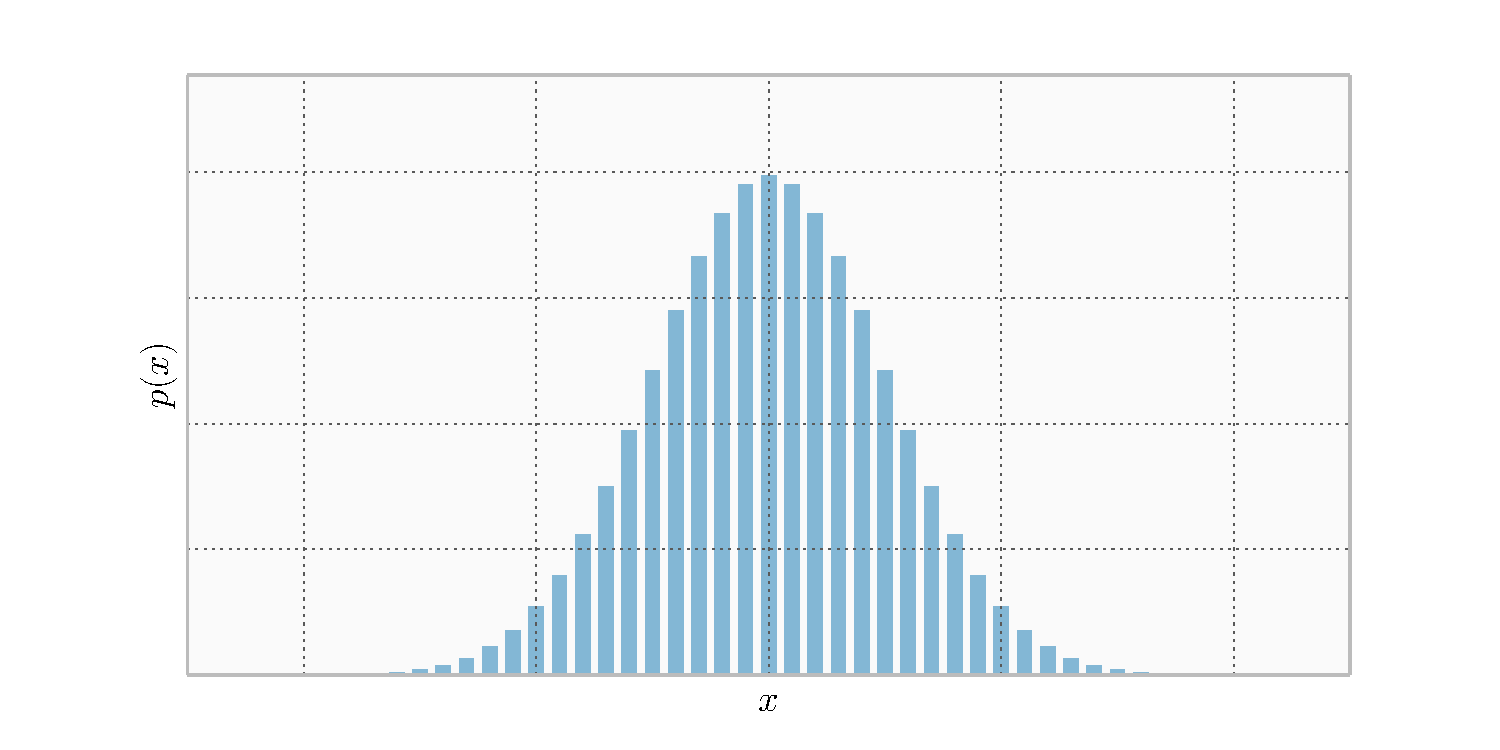
\includegraphics[width=10cm]{figure/binom.pdf}
\end{center}
\caption{A binomial distribution.}
\label{f:binomial}
\end{figure}

The binomial coefficient $\binom{n}{x}$ counts the number of distinct orderings in which exactly $x$ successes can occur among $n$ trials. This distribution arises naturally in many applied contexts: for example, modeling the number of defective items in a batch of size $n$, or the number of heads in $n$ tosses of a biased coin.

Since a Binomial random variable can be written as the sum of $n$ independent Bernoulli variables, its expectation and variance follow directly from linearity:
\begin{myalign}
\me{x} &= np,\\
\va{x} &= np(1-p).
\end{myalign}
Both quantities scale linearly with the number of trials, reflecting the accumulation of randomness across repeated experiments. As $n$ grows large, by the Central Limit Theorem, the Binomial distribution is well approximated by a Gaussian with the same mean and variance.

\subsection*{The Poisson Distribution}

The \alert{Poisson distribution} is used to model counts of events occurring randomly over a fixed interval of time or space, under the assumption that events occur independently and at a constant average rate. For $x \in \{0,1,2,\ldots\}$, we say $x \sim \text{Poisson}(\lambda)$ if
\begin{myequation}
p(x) = e^{-\lambda}\frac{\lambda^{x}}{x!},
\end{myequation}
where $\lambda > 0$ represents the expected number of events in the interval of interest.

\begin{figure}[ht]
\begin{center}
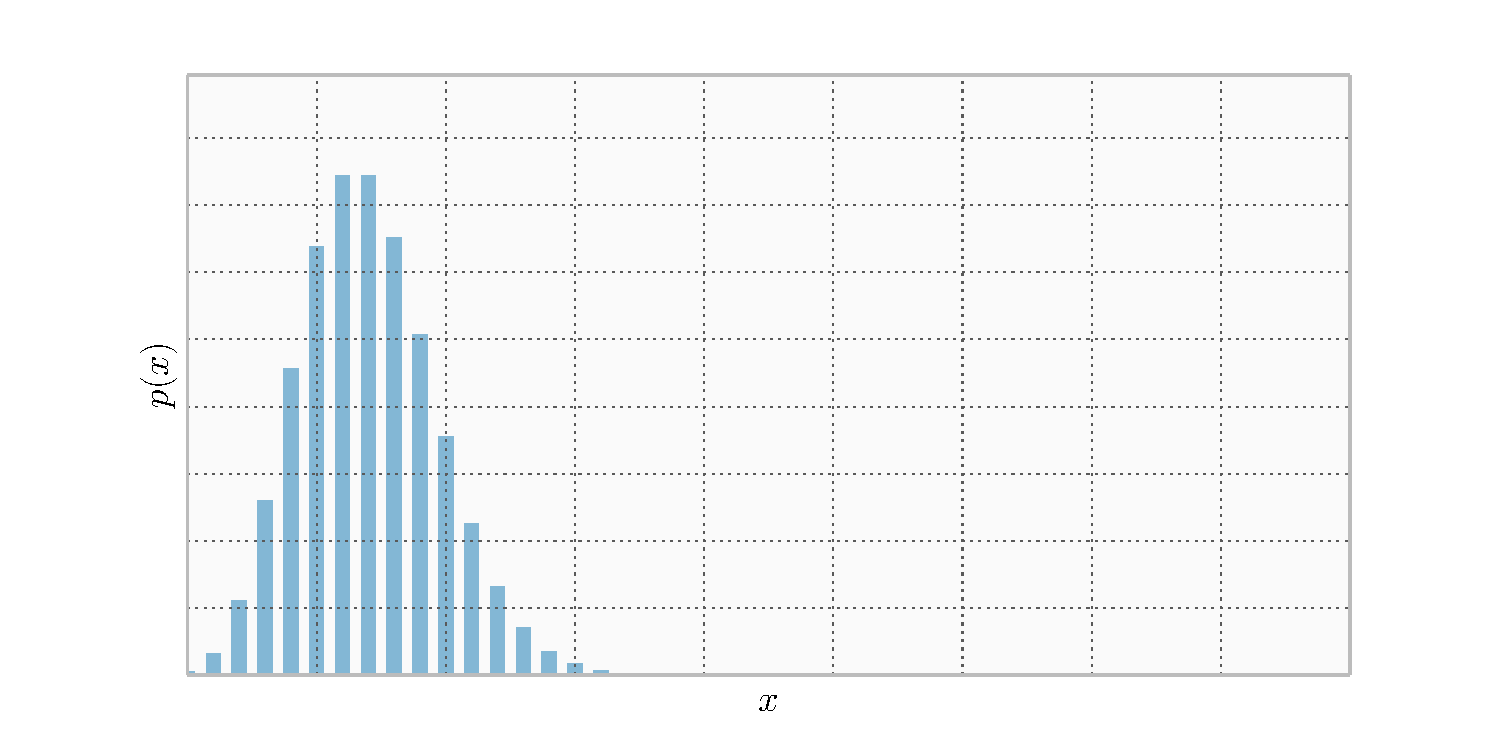
\includegraphics[width=10cm]{figure/poisson.pdf}
\end{center}
\caption{A Poisson distribution.}
\label{f:poisson}
\end{figure}

Typical applications include modeling the number of phone calls received by a call center in an hour, the number of radioactive decays detected in a fixed time window, or the number of emails arriving in a given period. From a theoretical standpoint, the Poisson distribution arises as a limiting case of the Binomial when the number of trials $n$ is large and the success probability $p$ is small, with the product $np = \lambda$ held constant. This derivation explains its appropriateness for modeling rare events in large populations.

A distinctive feature of the Poisson distribution is that its mean and variance coincide:
\begin{myequation}
\me{x} = \lambda,
\qquad
\va{x} = \lambda.
\end{myequation}
This \emph{equidispersion} property is often used in practice as a diagnostic: if observed count data exhibit a variance substantially different from the mean, the Poisson assumption may be inadequate and overdispersed alternatives (such as the negative binomial) may be more appropriate.

\subsection*{The Normal (Gaussian) Distribution}

Among continuous distributions, the \alert{Normal} or \alert{Gaussian distribution} occupies a central position. Its importance is largely due to the Central Limit Theorem, which states that sums of many independent random variables tend to follow a Gaussian distribution regardless of the original distributions. A continuous random variable $x \in \mathbb{R}$ follows a Normal distribution with mean $\mu$ and variance $\sigma^2$, written $x \sim \mathcal{N}(\mu,\sigma^2)$, if its probability density function is
\begin{myequation}
f(x) = \frac{1}{\sqrt{2\pi}\sigma}
       e^{-\frac{(x-\mu)^2}{2\sigma^2}}.
\end{myequation}

\begin{figure}[ht]
\begin{center}
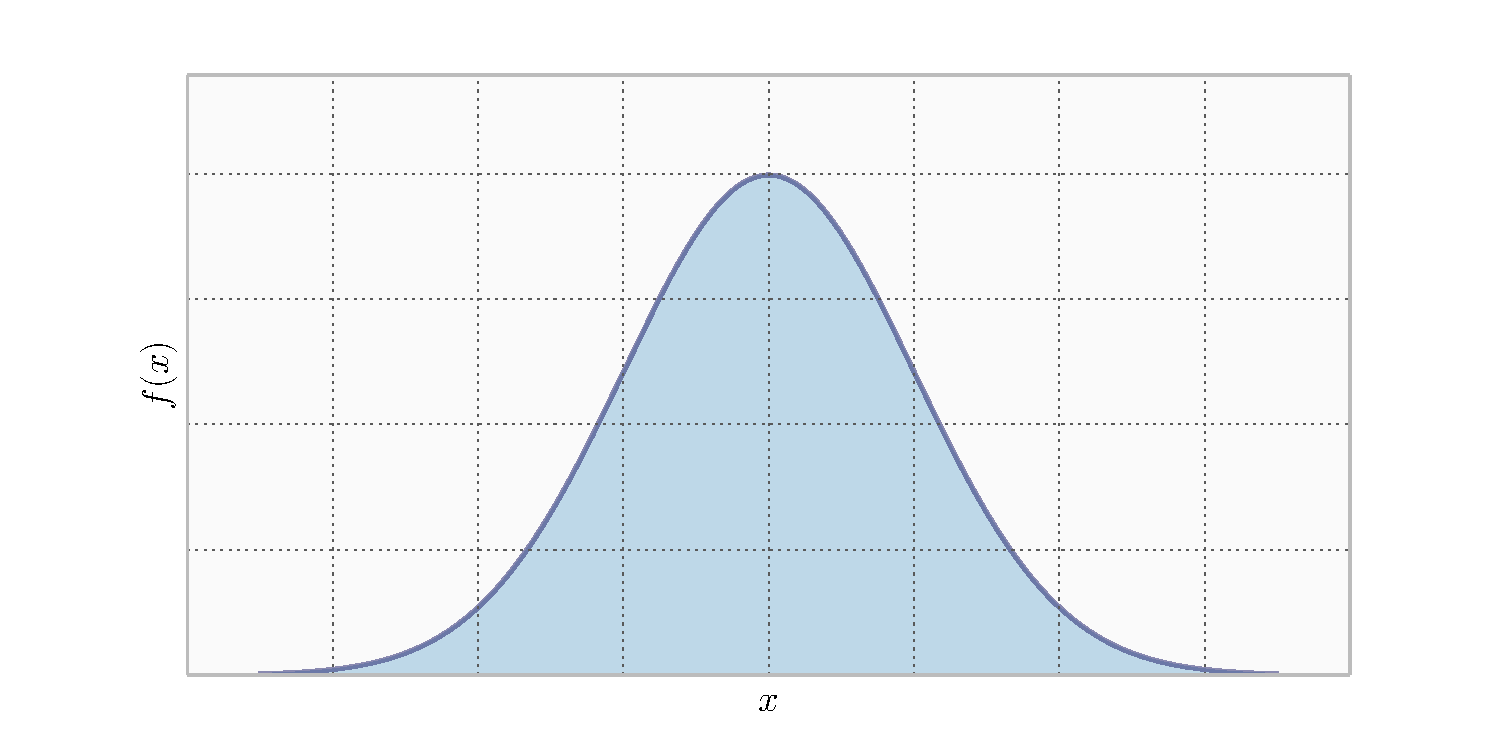
\includegraphics[width=10cm]{figure/normal.pdf}
\end{center}
\caption{A normal distribution.}
\label{f:gaussian}
\end{figure}

The parameter $\mu$ determines the location of the distribution while $\sigma$ controls its spread. The mean and variance of a Gaussian random variable coincide directly with these parameters, $\me{x} = \mu$ and $\va{x} = \sigma^2$, and the distribution is completely determined by these first two moments. A well-known empirical rule states that approximately $68\%$ of the probability mass lies within one standard deviation of the mean, and about $95\%$ within two standard deviations---a fact frequently used as a heuristic for identifying outliers.

\subsection*{The Beta Distribution}

The \alert{Beta distribution} is a flexible continuous distribution defined on the interval $[0,1]$. Because of this bounded support, it is particularly useful for modeling probabilities themselves, and in Bayesian statistics it serves as a conjugate prior for the parameter $p$ of Bernoulli and Binomial models (a concept developed at length later in this chapter). For $x \in [0,1]$, we say $x \sim \text{Beta}(\alpha,\beta)$ if its density is
\begin{myequation}
f(x) =
\frac{\Gamma(\alpha+\beta)}{\Gamma(\alpha)\Gamma(\beta)}
x^{\alpha-1}(1-x)^{\beta-1},
\end{myequation}
where $\alpha>0$ and $\beta>0$ are shape parameters, and $\Gamma(\cdot)$ denotes the Gamma function, which generalizes the factorial via $\Gamma(n)=(n-1)!$ for positive integers.

The parameters $\alpha$ and $\beta$ strongly influence the shape of the distribution. When $\alpha=\beta=1$, the distribution reduces to the Uniform distribution on $[0,1]$. When $\alpha=\beta>1$, the density is symmetric around $0.5$ and increasingly concentrated there. Larger values of $\alpha$ relative to $\beta$ concentrate mass near $1$, while larger values of $\beta$ relative to $\alpha$ concentrate mass near $0$.

\begin{figure}[t]
\centering
\begin{tabular}{cc}
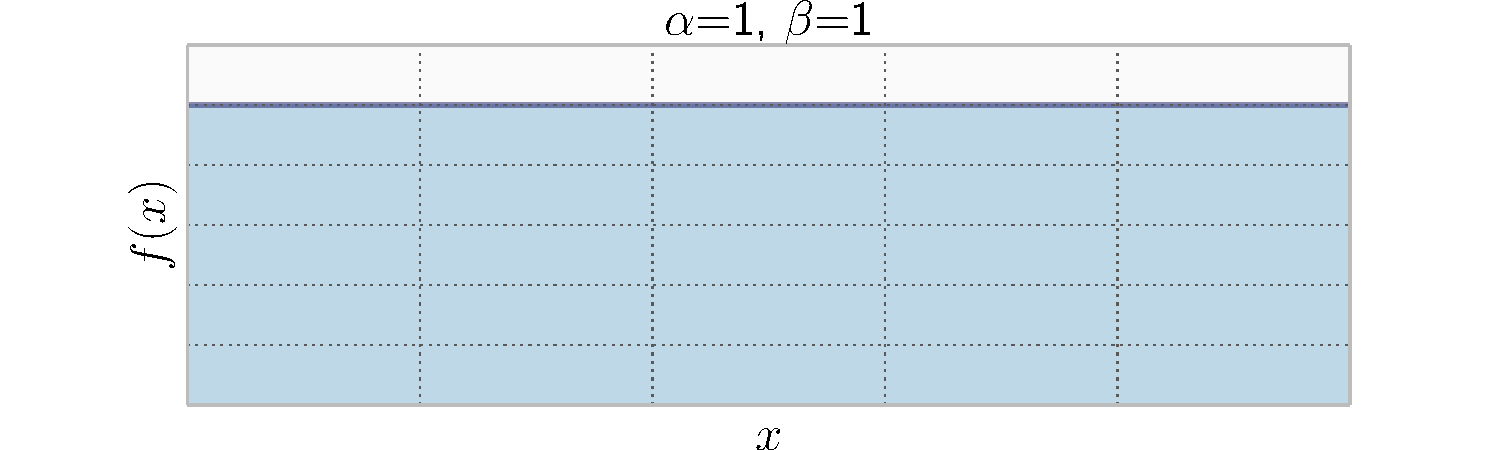
\includegraphics[width=0.48\linewidth]{figure/beta11.pdf} &
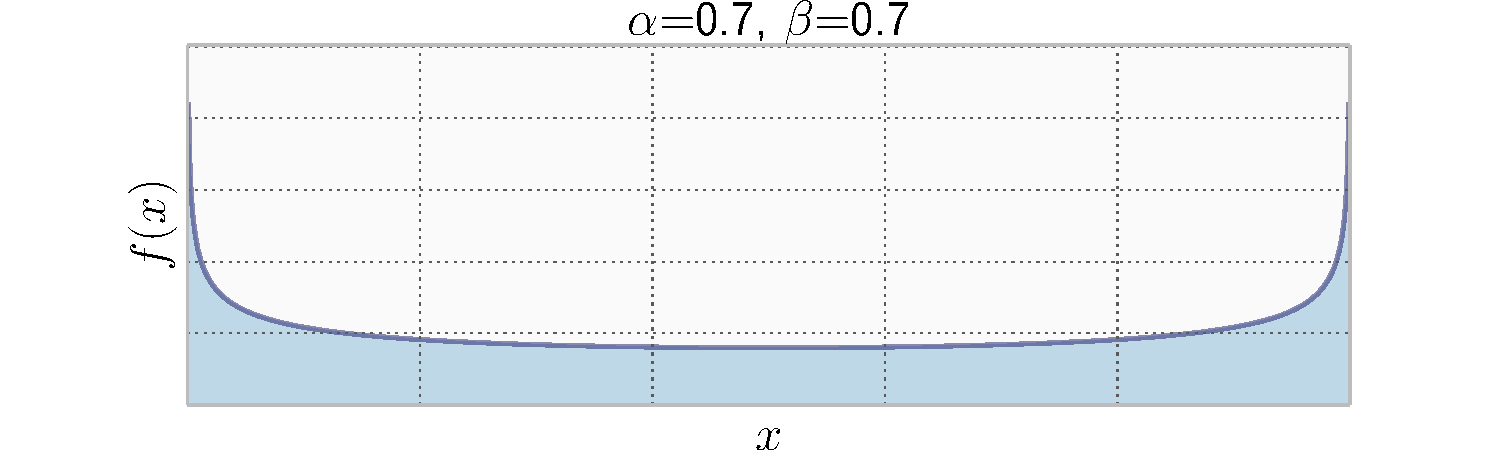
\includegraphics[width=0.48\linewidth]{figure/beta0707.pdf} \\
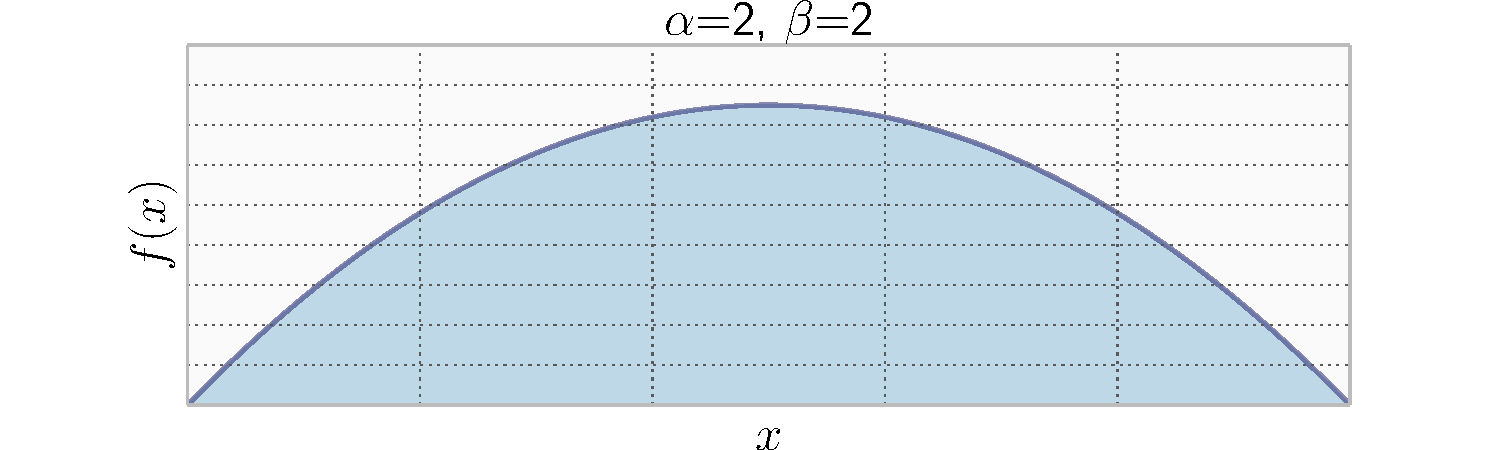
\includegraphics[width=0.48\linewidth]{figure/beta22.pdf} &
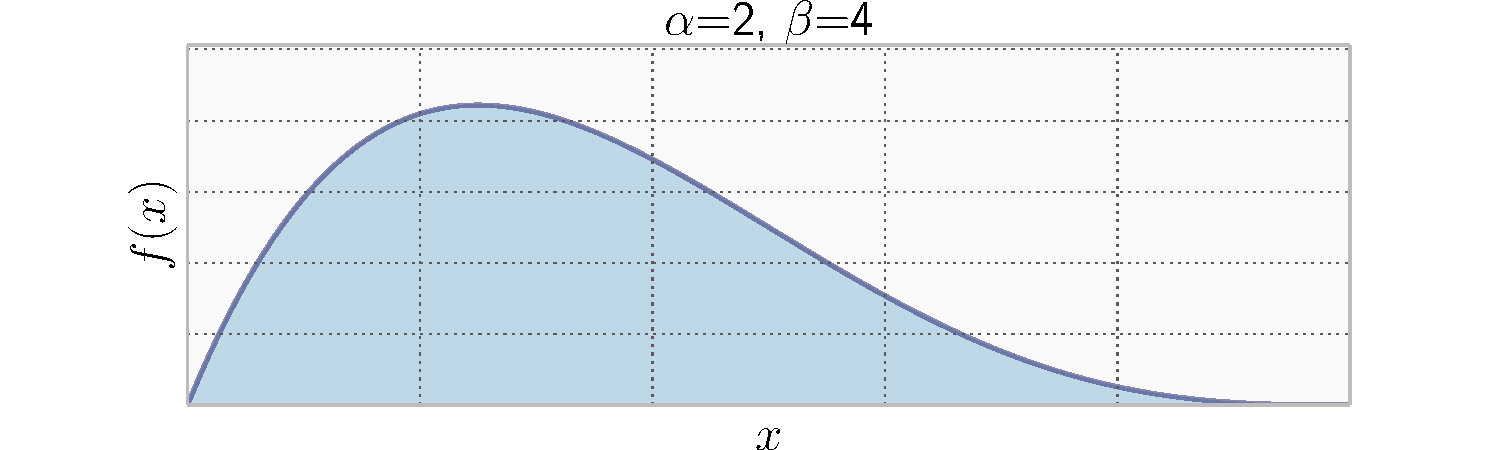
\includegraphics[width=0.48\linewidth]{figure/beta24.pdf} \\
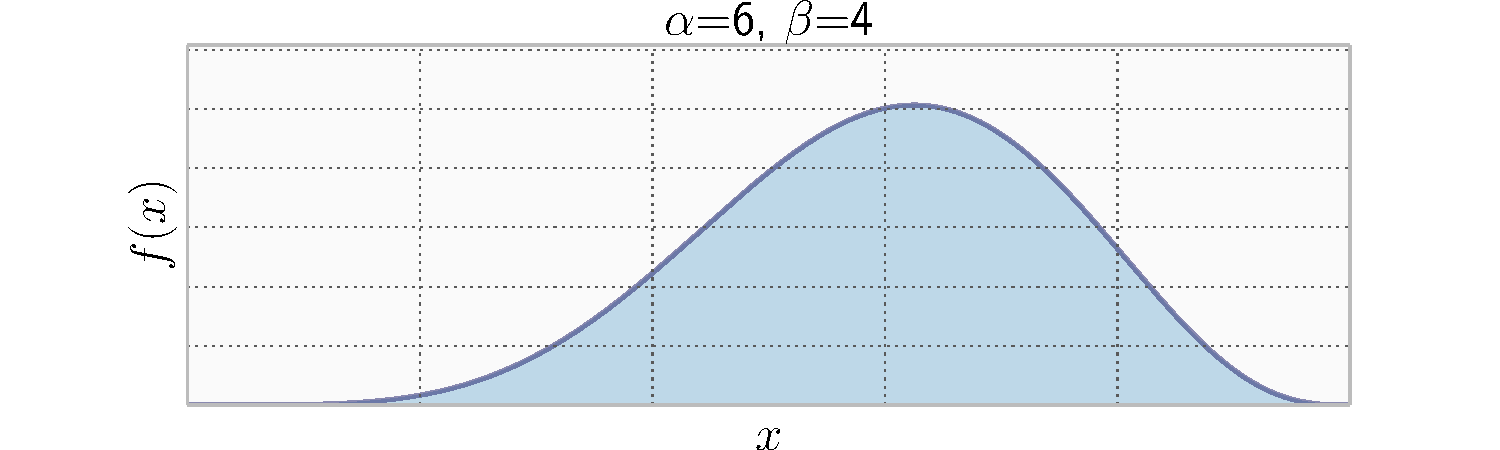
\includegraphics[width=0.48\linewidth]{figure/beta64.pdf} &
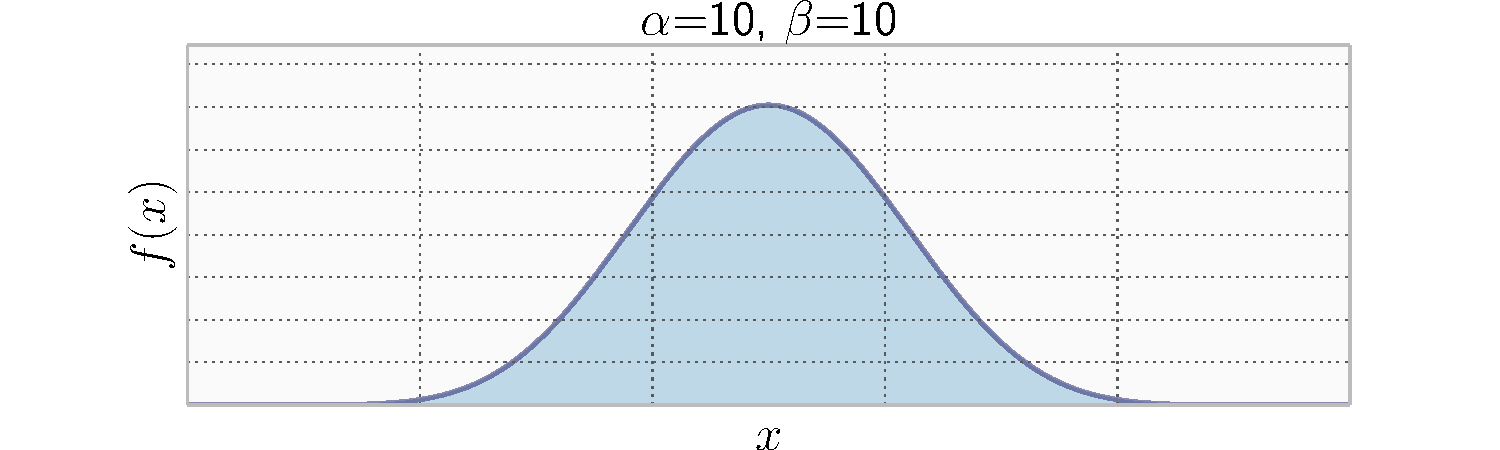
\includegraphics[width=0.48\linewidth]{figure/beta1010.pdf} \\
\end{tabular}
\caption{Different shapes of the Beta distribution.}
\label{f:beta}
\end{figure}

The expectation and variance of a Beta-distributed random variable have closed-form expressions:
\begin{myalign}
\me{x} &= \frac{\alpha}{\alpha+\beta},\\
\va{x} &= \frac{\alpha\beta}{(\alpha+\beta)^2(\alpha+\beta+1)}.
\end{myalign}
The mean $\alpha/(\alpha+\beta)$ has a natural interpretation: if $\alpha$ and $\beta$ are viewed as counts of prior successes and failures respectively, then the mean corresponds to the expected proportion of successes. This interpretation underlies the widespread use of the Beta distribution as a conjugate prior for Bernoulli and Binomial likelihoods, as elaborated in the section on Bayesian inference below.


\section*{Multivariate Probability and Random Vectors}

In most real-world problems, uncertainty does not concern a single quantity in isolation. Several random quantities interact simultaneously: measurements may be collected jointly, causes and effects may be intertwined, and predictions often depend on multiple features at once. For this reason, probability theory must be extended from single random variables to collections of variables described jointly. The natural mathematical object that captures such a collection is a \alert{random vector}, and the central tool for describing it is the \alert{joint distribution}.

\subsection*{Joint Distributions}

Consider first two discrete random variables $X$ and $Y$. Their joint distribution $p(x,y)$ assigns a probability to every pair of outcomes $(x,y)$, interpreted as the probability that $X=x$ and $Y=y$ occur simultaneously. As in the univariate case, a valid joint probability mass function must satisfy the basic axioms: probabilities are non-negative and the total probability over the entire sample space equals one,
\begin{myequation}
0 \le p(x,y) \le 1,
\qquad
\sum_{x\in V_X}\sum_{y\in V_Y} p(x,y)=1,
\end{myequation}
where $V_X$ and $V_Y$ denote the (discrete) value sets of $X$ and $Y$.

When $X$ and $Y$ are continuous, probabilities are assigned not to single points but to regions in the plane. It is convenient to start from the \alert{joint cumulative distribution function}
\begin{myequation}
F(x,y)=P(X\le x,\;Y\le y),
\end{myequation}
which measures the probability mass accumulated in the lower-left quadrant determined by $(x,y)$. If $F(x,y)$ is sufficiently smooth, the \alert{joint probability density function} is obtained by differentiating with respect to both variables:
\begin{myequation}
f(x,y)=\frac{\partial^2 F(x,y)}{\partial x\,\partial y}.
\end{myequation}
Geometrically, $f(x,y)$ can be visualized as a surface over the $(x,y)$-plane. If $A$ is any region in the plane, the probability that $(X,Y)$ falls in $A$ is obtained by integrating the density over that region:
\begin{myequation}
P\big((X,Y)\in A\big)=\iint_A f(x,y)\,dx\,dy.
\end{myequation}
In this sense, joint densities generalize the univariate idea that probability is ``area under the curve'': in two dimensions, probability becomes ``volume under the surface.''

\subsection*{Covariance and Correlation}

Once joint distributions are introduced, a natural question is how to summarize the \emph{dependence} between variables. The most common summary is \alert{covariance}, which measures whether two variables tend to deviate from their means in the same direction. If large values of $X$ tend to coincide with large values of $Y$, the covariance is positive; if they tend to go in opposite directions, it is negative. Formally, the covariance between $X$ and $Y$ is defined as the expected product of centered variables:
\begin{myequation}
\cov{X,Y}=\me{(X-\me{X})(Y-\me{Y})}.
\end{myequation}
Expanding the product and using linearity of expectation yields the computationally convenient identity
\begin{myequation}
\cov{X,Y}=\me{XY}-\me{X}\me{Y},
\end{myequation}
which compares the expectation of the product $XY$ with the product of the individual expectations. A particularly important consequence involves the variance of sums: using the definition of variance and expanding,
\begin{myequation}
\va{X+Y}=\va{X}+\va{Y}+2\cov{X,Y}.
\end{myequation}
This shows that the spread of $X+Y$ depends not only on the individual spreads of $X$ and $Y$, but also on how they co-vary. If $X$ and $Y$ are independent, their covariance is zero and the variance of the sum equals the sum of the variances. The converse, however, is not always true: zero covariance rules out only \emph{linear} dependence, and variables may exhibit nonlinear relationships while remaining uncorrelated.

A drawback of covariance is that it depends on the measurement units of $X$ and $Y$. To obtain a scale-free measure, covariance is normalized by the product of the standard deviations, yielding the \alert{Pearson correlation coefficient}:
\begin{myequation}
\rho_{X,Y}=\frac{\cov{X,Y}}{\sqrt{\va{X}\va{Y}}}.
\end{myequation}
By construction, $\rho_{X,Y}\in[-1,1]$. Values near $\pm 1$ indicate strong linear association, while values near $0$ indicate weak or absent linear dependence.

\subsection*{Random Vectors and Matrices}

When more than two variables are involved, linear algebra provides an efficient language for multivariate probability. A \alert{random vector} $\x$ is a column vector whose entries are random variables:
\begin{myequation}
\x=
\vcol{X_1}{X_2}{X_n}.
\end{myequation}
The expectation of a random vector is defined componentwise, so the mean of $\x$ is the vector $\Vmu = \me{\x}$ with $i$-th entry $\me{X_i}$.

The multivariate analogue of variance is the \alert{covariance matrix}, which collects the variances and pairwise covariances of all components into a single symmetric matrix:
\begin{myalign}
\VSigma
&=\me{(\x-\Vmu)(\x-\Vmu)^T}
=\me{\x\x^T}-\Vmu\Vmu^T.
\end{myalign}
The diagonal entries $\Sigma_{ii}$ are the variances $\va{X_i}$, while the off-diagonal entries $\Sigma_{ij}$ are the covariances $\cov{X_i,X_j}$. This matrix encodes how uncertainty is distributed across directions in $\mathbb{R}^n$. Indeed, for any fixed vector $a\in\mathbb{R}^n$, the linear combination $a^T\x$ has variance
\begin{myequation}
\va{a^T\x}=a^T\VSigma\,a,
\end{myequation}
and since variances must be non-negative for all $a$, it follows that $\VSigma$ must be \emph{positive semi-definite}. One can also define a \alert{correlation matrix} by standardizing each component and computing its covariance matrix; the result has ones on the diagonal and Pearson correlation coefficients off-diagonal.

\subsection*{The Multinomial Distribution}

The Binomial distribution models the number of successes in $n$ repetitions of a Bernoulli trial. When there are more than two possible outcomes, the appropriate generalization is the \alert{Multinomial distribution}. Suppose an experiment has $k$ possible outcomes with probabilities $p_1,\ldots,p_k$ satisfying $\sum_{i=1}^k p_i=1$, and perform $n$ independent trials, letting $x_i$ be the count of outcome $i$. The joint probability of the count vector $(x_1,\ldots,x_k)$ is
\begin{myequation}
p(x_1,\ldots,x_k)
=
\frac{n!}{x_1!\cdots x_k!}\prod_{i=1}^k p_i^{x_i},
\end{myequation}
subject to $\sum_{i=1}^k x_i=n$. The factorial term counts how many distinct orderings of the $n$ trials give rise to the same histogram $(x_1,\ldots,x_k)$. Each individual count $x_i$ behaves marginally like a Binomial variable, so $\me{x_i}=np_i$ and $\va{x_i}=np_i(1-p_i)$. However, the components exhibit an important dependence: since the total is fixed at $n$, increasing one count must reduce at least one other, inducing negative covariances between different categories.

\subsection*{The Dirichlet Distribution}

The Multinomial distribution models randomness in counts when the category probabilities $p_1,\ldots,p_k$ are assumed fixed. In many Bayesian settings, however, these probabilities are themselves unknown, and we wish to represent uncertainty about them. The Beta distribution serves this purpose for a single probability; its multivariate generalization, appropriate for a \emph{vector} of probabilities, is the \alert{Dirichlet distribution}.

A random vector $\x=(x_1,\ldots,x_k)$ follows a Dirichlet distribution with parameters $\alpha_1,\ldots,\alpha_k$, written $\x\sim\text{Dirichlet}(\alpha_1,\ldots,\alpha_k)$, if its density is
\begin{myequation}
f(x_1,\ldots,x_k)
=
\frac{1}{\Delta(\alpha_1,\ldots,\alpha_k)}\prod_{i=1}^k x_i^{\alpha_i-1},
\end{myequation}
with normalizing constant
\begin{myequation}
\Delta(\alpha_1,\ldots,\alpha_k)
=
\frac{\prod_{i=1}^k \Gamma(\alpha_i)}{\Gamma\!\left(\sum_{i=1}^k \alpha_i\right)}.
\end{myequation}
The defining constraint is that $\x$ lies on the \alert{$(k-1)$-dimensional simplex}: each $x_i\ge 0$ and $\sum_{i=1}^k x_i=1$. A Dirichlet random vector is therefore a random probability vector, where each component represents a proportion. Geometrically, for $k=3$ the simplex is a triangle, so Dirichlet samples can be visualized as points on a triangular region.

The parameters $\alpha_i$ are called \emph{concentration parameters} because they determine how mass is distributed over the simplex. When all parameters are equal ($\alpha_i=\alpha$), the distribution is symmetric and no category is preferred a priori. For $\alpha<1$, mass concentrates near the corners of the simplex, meaning draws are typically sparse---most categories receive near-zero probability. For $\alpha>1$, mass concentrates near the center, so draws tend to assign similar probabilities to all categories. The boundary case $\alpha=1$ corresponds to a uniform distribution over the simplex.

Denoting the total concentration $\alpha_0=\sum_{j=1}^k \alpha_j$, the mean and variance of each component have closed forms:
\begin{myequation}
\me{x_i}=\frac{\alpha_i}{\alpha_0},
\hspace{1cm}
\va{x_i}=\frac{\alpha_i(\alpha_0-\alpha_i)}{\alpha_0^2(\alpha_0+1)}.
\end{myequation}
The mean depends only on the relative proportions of the parameters, while the variance decreases as $\alpha_0$ increases: even if the proportions $\alpha_i/\alpha_0$ remain fixed, raising $\alpha_0$ concentrates the distribution more tightly around the mean. For this reason, $\alpha_0$ is often interpreted as a measure of overall confidence or the strength of prior information. In the symmetric case, all components share the mean $1/K$ and the variance
\begin{myequation}
\va{x_i}=\frac{K-1}{K^2(K\alpha+1)},
\end{myequation}
which makes the concentration effect particularly transparent.

Visual intuition is especially helpful for the Dirichlet distribution. When $k=3$, the density can be plotted over the triangular simplex. For small parameters ($\alpha_i<1$) the density peaks near corners; for $\alpha_i=1$ it is uniform; for $\alpha_i>1$ it concentrates near the center.

\begin{figure}[t]
\centering
\begin{tabular}{ccc}

\includegraphics[width=0.30\linewidth]{dirichlet1.pdf} &

\includegraphics[width=0.30\linewidth]{dirichlet2.pdf} &

\includegraphics[width=0.30\linewidth]{dirichlet3.pdf}
\end{tabular}
\caption{Different shapes of the Dirichlet distribution.}
\label{f:dirichlet}
\end{figure}

A final reason for the importance of the Dirichlet distribution is its \alert{conjugacy} with the Multinomial. If we place a Dirichlet prior on the unknown probability vector and then observe Multinomial data (counts across categories), the posterior is also Dirichlet with updated parameters. This property makes Bayesian inference analytically tractable and explains why Dirichlet priors are ubiquitous in models requiring uncertainty over categorical probability vectors, from mixture models to topic modeling.


\section*{The Normal Distribution}

The \alert{Normal}, or \alert{Gaussian} distribution is arguably the most influential probability model in statistics, signal processing, and machine learning. Its prominence is not merely historical: it arises naturally in a wide range of contexts and enjoys a set of algebraic properties that make it exceptionally convenient for both theoretical analysis and practical computation.

A major reason for its ubiquity is the \alert{Central Limit Theorem}, which informally states that when many independent (or weakly dependent) random contributions are added together, the resulting sum tends to exhibit a Gaussian shape, largely regardless of the detailed form of the individual contributions. In applied terms, this explains why measurement noise, aggregate effects, and many macroscopic quantities appear approximately Normal. At the same time, the Gaussian behaves well under many operations that frequently arise in modeling: linear transformations preserve Gaussianity, products of Gaussian densities remain Gaussian up to normalization, and convolutions (which correspond to sums of independent variables) yield another Gaussian. These are exactly the properties that make Gaussians the default choice in regression, state-space models, and probabilistic graphical models.

\subsection*{The Univariate Case}

A real-valued random variable $x\in\mathbb{R}$ is said to be Gaussian with mean $\mu$ and variance $\sigma^2$, written $x\sim\mathcal{N}(\mu,\sigma^2)$, if its density has the familiar bell-shaped form
\begin{myalign}
p(x) &= \mathcal{N}(\mu,\sigma^2)
= \frac{1}{\sqrt{2\pi}\sigma}\exp\!\left(-\frac{(x-\mu)^2}{2\sigma^2}\right).
\end{myalign}
The mean $\mu$ specifies the center of the distribution and the variance $\sigma^2$ controls its spread. The Gaussian is completely determined by these first two moments: once $\mu$ and $\sigma^2$ are given, the entire distribution is fixed. A classical and practically useful consequence is the concentration of probability around the mean: approximately $68\%$ of the mass lies in the interval $|x-\mu|\le \sigma$, and about $95\%$ within $|x-\mu|\le 2\sigma$. This empirical rule is frequently used as a heuristic for identifying outliers in data assumed to follow a Gaussian noise model.

\subsection*{The Multivariate Gaussian}

In modern applications, data are rarely one-dimensional. When we model a random vector $\x\in\mathbb{R}^d$, the Gaussian generalizes by replacing the scalar mean with a mean vector $\Vmu\in\mathbb{R}^d$ and the scalar variance with a $d\times d$ \alert{covariance matrix} $\VSigma$:
\begin{myalign}
p(\x) &= \mathcal{N}(\Vmu,\VSigma)
= \frac{1}{(2\pi)^{d/2}|\VSigma|^{1/2}}
\exp\!\left(-\frac{1}{2}(\x-\Vmu)^T\VSigma^{-1}(\x-\Vmu)\right).
\end{myalign}
Here $|\VSigma|$ denotes the determinant of $\VSigma$, and $\VSigma^{-1}$ its inverse (assuming $\VSigma$ is non-singular). The diagonal entries of $\VSigma$ are the variances of the individual components, while the off-diagonal entries encode pairwise covariances. In this sense, $\VSigma$ expresses the internal geometry of the distribution.

The exponent in the multivariate Gaussian is a quadratic form, which reveals the geometric structure of the distribution. Define the \alert{Mahalanobis distance} from $\x$ to the mean as
\begin{myalign}
\Delta^2 = (\x-\Vmu)^T\VSigma^{-1}(\x-\Vmu).
\end{myalign}
This distance accounts for both scale and correlation. Unlike the Euclidean distance $\|\x-\Vmu\|$, which treats all directions equally, the Mahalanobis distance rescales directions according to the covariance: directions with large variance are stretched (so deviations are less surprising), while directions with small variance are compressed. Because the density depends on $\x$ only through $\Delta^2$, sets of constant density form ellipsoids centered at $\Vmu$. In the special case $\VSigma=\mathbf{I}$, these reduce to spheres, recovering the isotropic Gaussian where all directions are equivalent.

\subsubsection*{Spectral Decomposition and Principal Axes}

To understand the orientation and shape of the Gaussian ellipsoids, it is useful to examine the spectral decomposition of $\VSigma$. Since $\VSigma$ is symmetric and positive semi-definite, it admits an orthonormal eigen-decomposition with eigenvectors $\mathbf{u}_i$ and eigenvalues $\lambda_i\ge 0$:
\begin{myequation}
\VSigma=\sum_{i=1}^{d}\lambda_i \mathbf{u}_i\mathbf{u}_i^T
\qquad\Longrightarrow\qquad
\VSigma^{-1}=\sum_{i=1}^{d}\frac{1}{\lambda_i}\mathbf{u}_i\mathbf{u}_i^T.
\end{myequation}
The eigenvectors $\mathbf{u}_i$ define the principal axes of the ellipsoids, while the eigenvalues $\lambda_i$ determine the variances along those axes. Rotating into the eigenvector basis by defining $y_i = \mathbf{u}_i^T(\x-\Vmu)$, the quadratic form diagonalizes:
\begin{myequation}
(\x-\Vmu)^T\VSigma^{-1}(\x-\Vmu)=\sum_{i=1}^d \frac{y_i^2}{\lambda_i},
\end{myequation}
and the density factorizes into a product of one-dimensional Gaussians:
\begin{myequation}
f(\x|\Vmu,\VSigma)=\prod_{i=1}^{d}\frac{1}{\sqrt{2\pi\lambda_i}}
\exp\!\left(-\frac{1}{2}\frac{y_i^2}{\lambda_i}\right).
\end{myequation}
This factorization illustrates a key insight: correlations in the original coordinates disappear after an appropriate rotation. Each eigenvalue $\lambda_i$ can be read as the variance along direction $\mathbf{u}_i$, so large eigenvalues correspond to directions of high spread and small eigenvalues to directions of tight concentration.

\subsection*{Conditioning and Marginalization}

One of the most powerful properties of multivariate Gaussians is their stability under taking marginals and conditionals. In multivariate problems, we often need to ignore some variables (marginalization) or update beliefs after observing others (conditioning). For general distributions these operations can produce complicated forms, but for Gaussians they yield Gaussian results with parameters expressible in closed form.

Partitioning the random vector into two blocks,
\begin{myequation}
\x=
\begin{pmatrix}
\x_1\\
\x_2
\end{pmatrix},
\qquad
\Vmu=
\begin{pmatrix}
\Vmu_1\\
\Vmu_2
\end{pmatrix},
\qquad
\VSigma=
\begin{pmatrix}
\VSigma_{11} & \VSigma_{12}\\
\VSigma_{21} & \VSigma_{22}
\end{pmatrix},
\end{myequation}
with $\VSigma_{21}=\VSigma_{12}^T$, the marginal distribution of $\x_1$ alone is simply
\begin{myequation}
p(\x_1)=\mathcal{N}(\Vmu_1,\VSigma_{11}).
\end{myequation}
This means the behavior of a subset of jointly Gaussian variables is determined entirely by the corresponding subvector of means and the corresponding principal submatrix of the covariance---the other variables can be ignored without any further calculation. The conditional distribution of $\x_1$ given an observed value of $\x_2$, on the other hand, is also Gaussian but with an updated mean and a reduced covariance:
\begin{myalign}
\Vmu_{1|2} &= \Vmu_1-\VSigma_{12}\VSigma_{22}^{-1}(\x_2-\Vmu_2),\\
\VSigma_{1|2} &= \VSigma_{11}-\VSigma_{12}\VSigma_{22}^{-1}\VSigma_{21}.
\end{myalign}
The correction term $\VSigma_{12}\VSigma_{22}^{-1}(\x_2-\Vmu_2)$ adjusts the mean according to how $\x_1$ co-varies with $\x_2$: when the two blocks are strongly correlated, observing $\x_2$ shifts the mean estimate of $\x_1$ substantially. The conditional covariance $\VSigma_{1|2}$ is smaller (in the positive semi-definite sense) than $\VSigma_{11}$, reflecting the reduction in uncertainty about $\x_1$ once $\x_2$ is known.

\subsection*{Bayesian Inference with Gaussians}

Gaussians are exceptionally convenient in Bayesian inference because assuming Gaussian priors and Gaussian likelihoods guarantees that the posterior remains Gaussian. This phenomenon is sometimes described as the Gaussian being \alert{self-conjugate} under linear-Gaussian observation models.

Consider a Gaussian prior on $\x$ and a Gaussian likelihood for observations $\y$ given $\x$:
\begin{myalign}
\text{Prior: } \gaussiandistr{\x}{\Vmu}{\VSigma_1}
\qquad
\text{Likelihood: } \gaussiandistr{\y|\x}{\A\x+\b}{\VSigma_2}.
\end{myalign}
The likelihood expresses that $\y$ is generated from a linear transformation of $\x$ plus Gaussian noise with covariance $\VSigma_2$. Under these assumptions, the posterior $p(\x|\y)$ is Gaussian with parameters
\begin{myalign}
\hat{\Vmu}
&=
(\VSigma_1^{-1}+\A^T\VSigma_2^{-1}\A)^{-1}
\left(\A^T\VSigma_2^{-1}(\y-\b)+\VSigma_1^{-1}\Vmu\right),\\
\hat{\VSigma}
&=
(\VSigma_1^{-1}+\A^T\VSigma_2^{-1}\A)^{-1}.
\end{myalign}
These expressions illustrate a general Bayesian principle: the posterior precision matrix $\hat{\VSigma}^{-1}$ is the sum of the prior precision $\VSigma_1^{-1}$ and an information term $\A^T\VSigma_2^{-1}\A$ contributed by the data. Likewise, the posterior mean combines the prior mean and the data term, each weighted by their respective precisions. This closed-form updating rule is the mathematical foundation of \alert{Bayesian linear regression}, where $\x$ represents regression coefficients, and of \alert{Kalman filtering}, where $\x$ represents a latent state updated sequentially as observations arrive.


\section*{Bayesian Statistics}

The field of statistics is broadly divided into two main philosophical schools of thought: the \alert{frequentist} approach and the \alert{Bayesian} approach. In \textbf{classical (frequentist) statistics}, probability is strictly defined as the long-run frequency of an event over a sequence of identical, reproducible experiments. A model parameter $\Theta$ is viewed as a fixed but unknown constant, and there is no notion of a ``distribution'' for $\Theta$; the goal is simply to find a good point estimate. In contrast, \alert{Bayesian statistics} interprets probability as a \alert{degree of belief} or uncertainty about an event. Parameters are treated not as fixed constants, but as \textbf{random variables}, which allows us to quantify our uncertainty about them using the same mathematical language we use for the data.

The bridge between these two perspectives is \alert{Bayes' Rule}. For two random variables $X$ (the observed data) and $\Theta$ (the model parameters), it states
\begin{myequation}
p(\Theta=\theta|X=x)=\frac{p(X=x|\Theta=\theta)p(\Theta=\theta)}{p(X=x)}.
\end{myequation}
This equation is powerful because it relates the conditional probability of the parameter given the data---which is what we actually want to know---to the probability of the data given the parameter, which is what our scientific models typically provide.

\subsection*{The Process of Bayesian Inference}

When we perform Bayesian inference, we start with a probabilistic model $p(x|\Theta)$ and an observed dataset $\mathbf{X}$. Unlike frequentist methods that search for a single value of $\Theta$ that best fits the data, Bayesian inference seeks to compute the entire distribution of possible values for $\Theta$ after observing $\mathbf{X}$:
\begin{myequation}
p(\Theta|\mathbf{X})=\frac{p(\mathbf{X}|\Theta)p(\Theta)}{p(\mathbf{X})}.
\end{myequation}
To understand this formula, we must identify each of its four components. The \textbf{prior} $p(\Theta)$ represents our state of knowledge \alert{before} seeing any data; it encodes previous experiments, expert opinion, or a non-informative distribution when prior knowledge is scant. The \textbf{likelihood} $p(\mathbf{X}|\Theta)$ describes how well the observed data are explained by a specific parameter value, serving as the ``evidence'' provided by the current experiment. The \textbf{posterior} $p(\Theta|\mathbf{X})$ is the result of the inference---our updated knowledge \alert{after} observing $\mathbf{X}$, combining prior beliefs with the new evidence. Finally, the \textbf{evidence} $p(\mathbf{X})$, also called the marginal likelihood, is computed as $\int p(\mathbf{X}|\Theta')p(\Theta')d\Theta'$ and acts as a normalizing constant ensuring the posterior is a valid probability distribution. The posterior encapsulates everything a Bayesian model knows about $\Theta$ after observing the data: it supports point estimation (via the posterior mean or mode), uncertainty quantification (via credible intervals), and predictive inference (by integrating the likelihood over the posterior, as discussed in the chapter on sampling methods).

\subsection*{Conjugate Distributions}

One of the historical challenges of Bayesian statistics was that computing the posterior often required solving intractable integrals, specifically the evidence term $p(\mathbf{X})$. To simplify this, statisticians look for \alert{conjugate distributions}. A prior distribution $p(x)$ is said to be \textbf{conjugate} to a likelihood $p(y|x)$ if the resulting posterior $p(x|y)$ belongs to the same parametric family as the prior. The practical consequence is enormous: it allows Bayesian updates to be performed using simple algebraic rules rather than numerical integration. If our prior belief is expressed as a distribution of a certain type, and the posterior after observing data is of that same type, learning amounts to updating the parameters of that distribution according to explicit formulas.

\subsection*{Conjugate Priors: Examples}

The following examples develop the concept of conjugacy concretely for the most common models of discrete and continuous data.

\subsubsection*{The Beta-Bernoulli Model}

The simplest Bayesian model describes a single binary event, such as a coin toss, where we wish to estimate the probability $\phi$ of success. We place a \alert{Beta} prior over $\phi$:
\begin{myalign}
p(\phi|\alpha,\beta)&=\text{Beta}(\phi|\alpha,\beta)=\frac{\Gamma(\alpha+\beta)}{\Gamma(\alpha)\Gamma(\beta)}\phi^{\alpha-1}(1-\phi)^{\beta-1}.
\end{myalign}
For a single observation $x \in \{0, 1\}$ with \alert{Bernoulli} likelihood $p(x|\phi)=\phi^{x}(1-\phi)^{1-x}$, applying Bayes' rule and focusing on the proportionality in $\phi$ yields
\begin{myalign}
p(\phi|x) &\propto p(x|\phi)\,p(\phi|\alpha,\beta)
\propto \phi^{\alpha+x-1}(1-\phi)^{\beta+(1-x)-1}.
\end{myalign}
This is immediately recognizable as the kernel of a Beta distribution, so
\begin{myequation}
p(\phi|x) = \text{Beta}(\phi|\alpha+x,\; \beta+1-x).
\end{myequation}
The hyperparameters $\alpha$ and $\beta$ act as virtual counts of prior successes and failures. Observing a success increments $\alpha$ by one; observing a failure increments $\beta$ by one. This update rule has a transparent interpretation: the posterior mean $(\alpha+x)/(\alpha+\beta+1)$ interpolates between the prior mean $\alpha/(\alpha+\beta)$ and the observed proportion.

\subsubsection*{The Beta-Binomial Extension}

When we observe $N$ independent trials resulting in $k$ successes, the likelihood is \alert{Binomial}:
\begin{myalign}
p(k|\phi,N)&=\binom{N}{k}\phi^{k}(1-\phi)^{N-k}.
\end{myalign}
Multiplying the Beta prior by this likelihood and collecting powers of $\phi$ gives
\begin{myalign}
p(\phi|k,N,\alpha,\beta) &\propto \phi^{\alpha+k-1}(1-\phi)^{\beta+N-k-1},
\end{myalign}
which is recognized as the kernel of $\text{Beta}(\phi|\alpha+k,\;\beta+N-k)$. The normalization constant, which can be verified by the integral formula for the Beta function, is
\begin{myequation}
Z=\int_0^1\phi^{\alpha+k-1}(1-\phi)^{\beta+N-k-1}d\phi=\frac{\Gamma(\alpha+k)\Gamma(\beta+N-k)}{\Gamma(\alpha+\beta+N)}.
\end{myequation}
This confirms that $k$ observed successes and $N-k$ failures simply add to the prior pseudo-counts $\alpha$ and $\beta$.

\subsubsection*{The Multinomial and Dirichlet}

When the outcome space has $K$ categories, the Bernoulli/Binomial model generalizes to the \alert{Multinomial}. If we have $N$ observations with $N_j$ counts in category $j$, the likelihood (up to a constant in $\phi$) is
\begin{myequation}
p(\mathbf{X}|\phi_{1},\ldots,\phi_{K}) \propto \prod_{j=1}^{K}\phi_{j}^{N_{j}},
\end{myequation}
subject to $\sum \phi_j = 1$. The conjugate prior for the Multinomial parameters is the \alert{Dirichlet}:
\begin{myalign}
p(\Vphi|\Valpha) &= \frac{\Gamma(\sum \alpha_{i})}{\prod \Gamma(\alpha_{i})}\prod_{i=1}^{K}\phi_{i}^{\alpha_{i}-1}.
\end{myalign}

Given a Dirichlet prior $\text{Dir}(\Vphi|\Valpha)$ and observed counts $\mathbf{z} = (z_1, \ldots, z_K)$, the posterior follows by combining the prior and likelihood:
\begin{myalign}
p(\Vphi|\mathbf{z},\Valpha) &\propto \left( \prod_{i=1}^{K}\phi_{i}^{z_{i}} \right) \left( \prod_{i=1}^{K}\phi_{i}^{\alpha_{i}-1} \right)
= \prod_{i=1}^{K}\phi_{i}^{\alpha_i+z_i-1}.
\end{myalign}
This is the kernel of a new Dirichlet with updated parameters:
\begin{myequation}
p(\Vphi|\mathbf{z},\Valpha) = \text{Dir}(\Vphi | \Valpha + \mathbf{z}),
\end{myequation}
where $\Valpha' = (\alpha_{1}+z_1, \ldots, \alpha_{K}+z_K)$. The prior parameters $\alpha_i$ (representing the initial strength of belief in each category) are directly augmented by the observed counts $z_i$. This makes the Dirichlet-Multinomial model extremely efficient for high-dimensional problems such as Latent Dirichlet Allocation in text mining.

\subsubsection*{The Gaussian-Gaussian Conjugacy}

We now examine conjugacy for continuous variables. Consider a dataset $\mathbf{X} = \{x_1, \ldots, x_n\}$ sampled from a Gaussian with unknown mean $\mu$ but known variance $\sigma^2$. We represent prior uncertainty about $\mu$ through a Gaussian prior:
\begin{myequation}
p(\mu) = \mathcal{N}(\mu | \mu_0, \tau_0^2) = \frac{1}{\sqrt{2\pi\tau_0^2}} \exp\!\left( -\frac{(\mu - \mu_0)^2}{2\tau_0^2} \right).
\end{myequation}
For a single observation $x$, the likelihood is
\begin{myequation}
p(x | \mu) = \mathcal{N}(x | \mu, \sigma^2) = \frac{1}{\sqrt{2\pi\sigma^2}} \exp\!\left( -\frac{(x - \mu)^2}{2\sigma^2} \right).
\end{myequation}
According to Bayes' rule, the posterior $p(\mu | x)$ is proportional to the product of the prior and the likelihood. Since both are exponentials of quadratic forms in $\mu$, their product is also an exponential of a quadratic form, so the posterior must be Gaussian. Combining the exponents and collecting terms in $\mu$:
\begin{myalign}
p(\mu | x) &\propto p(x | \mu)\, p(\mu) \\
&\propto \exp\!\left( -\frac{(x-\mu)^2}{2\sigma^2} - \frac{(\mu-\mu_0)^2}{2\tau_0^2} \right).
\end{myalign}
Expanding the squares and regrouping terms in $\mu^2$ and $\mu$, the exponent becomes
\begin{myalign}
\text{Exponent} &= -\frac{1}{2} \left[ \mu^2 \left( \frac{1}{\sigma^2} + \frac{1}{\tau_0^2} \right) - 2\mu \left( \frac{x}{\sigma^2} + \frac{\mu_0}{\tau_0^2} \right) + \text{const} \right].
\end{myalign}
Completing the square in $\mu$, we identify the posterior as $\mathcal{N}(\mu | \mu_n, \tau_n^2)$ with parameters
\begin{myalign}
\frac{1}{\tau_n^2} &= \frac{1}{\tau_0^2} + \frac{1}{\sigma^2}, \\
\mu_n &= \tau_n^2 \left( \frac{\mu_0}{\tau_0^2} + \frac{x}{\sigma^2} \right).
\end{myalign}

To understand these update rules intuitively, it is helpful to introduce the concept of \alert{precision}, defined as the reciprocal of variance ($\beta = 1/\sigma^2$). The posterior precision is simply the sum of the prior precision and the data precision:
\begin{myequation}
\beta_n = \beta_0 + \beta_{\text{data}},
\end{myequation}
so observing data always increases certainty and decreases the posterior variance. The posterior mean is a \textbf{precision-weighted average} of the prior mean and the observation:
\begin{myequation}
\mu_n = \frac{\beta_0}{\beta_0 + \beta_{\text{data}}}\mu_0 + \frac{\beta_{\text{data}}}{\beta_0 + \beta_{\text{data}}}x.
\end{myequation}
If the prior is highly certain ($\beta_0$ large), the posterior mean remains close to $\mu_0$; if the data is precise or the prior is diffuse ($\beta_0$ small), the posterior is pulled strongly toward $x$. This interpolation between prior and data is a characteristic feature of all Bayesian updates.

When we have a full dataset $\mathbf{X} = \{x_1, \ldots, x_n\}$, the likelihood is the product of $n$ independent Gaussians, and the update rules generalize by accumulating information from all data points:
\begin{myalign}
\frac{1}{\tau_n^2} &= \frac{1}{\tau_0^2} + \frac{n}{\sigma^2}, \\
\mu_n &= \frac{\frac{1}{\tau_0^2}\mu_0 + \frac{n}{\sigma^2}\bar{x}}{\frac{1}{\tau_0^2} + \frac{n}{\sigma^2}},
\end{myalign}
where $\bar{x} = \frac{1}{n}\sum x_i$ is the sample mean. As $n \to \infty$, the influence of the prior mean $\mu_0$ vanishes, the posterior mean $\mu_n$ converges to the sample mean $\bar{x}$, and the posterior variance $\tau_n^2$ shrinks toward zero. This demonstrates the \alert{asymptotic consistency} of Bayesian estimation: with enough data, the evidence accumulated in the likelihood eventually overwhelms any initial prior belief, however strong.


\section*{Information Theory}

Information theory provides a rigorous mathematical language for formalizing the intuitive notion of \emph{information}. At its core lies a simple idea: an observation is informative to the extent that it is unexpected. Highly predictable events convey little new information, while rare events carry a great deal of it. Starting from this principle, information theory builds a coherent framework connecting probability, uncertainty, data compression, statistical inference, and learning.

\subsection*{Quantifying Surprise: The Information Measure}

Let $X$ be a discrete random variable with pmf $p(x)$. We seek a numerical quantity $h(x)$ capturing the amount of information, or level of \emph{surprise}, associated with observing $X = x$. Rather than postulating a definition arbitrarily, we require $h(x)$ to satisfy two natural principles. First, likely events should not be surprising and should therefore carry little information, while unlikely events should be highly informative: $h(x)$ must be a decreasing function of $p(x)$. Second, information should be additive for independent events: if two independent observations are made, the total information gained should be the sum of the individual informations, so $h(x,y) = h(x) + h(y)$ when $X \perp Y$.

These two requirements uniquely determine the functional form of $h(x)$ up to a choice of scale. The only function that converts products of probabilities into sums of information is the logarithm, leading to
\begin{myequation}
h(x) = -\log_b p(x),
\end{myequation}
where the base $b$ sets the unit of measurement. In information theory, the conventional choice is $b=2$, measuring information in \emph{bits}. For example, if $p(x)=1/2$, then $h(x)=1$ bit, corresponding to the information gained from observing the outcome of a fair coin toss.

\subsection*{Entropy: Average Uncertainty}

While $h(x)$ quantifies the information of a single outcome, it does not describe the uncertainty of the random variable as a whole. To capture this, we take the expectation of $h(x)$ over the distribution of $X$, defining the \alert{entropy}:
\begin{myequation}
H(X) = \mathbb{E}[h(x)] = -\sum_x p(x)\log_2 p(x).
\end{myequation}
Entropy measures the average number of bits required to describe the outcome of $X$. A distribution concentrated on a single outcome has zero entropy (no uncertainty), while a distribution spread across many outcomes has higher entropy. Among all discrete distributions with $k$ fixed outcomes, the uniform distribution achieves the maximum entropy, since all outcomes are equally unpredictable. Since $p(x)\in[0,1]$ implies $\log_2 p(x)\leq 0$, entropy is always non-negative, and the lower bound $H(X)=0$ is attained if and only if $p(x)=1$ for some outcome $x$.

\subsection*{Maximum Entropy Principle}

A fundamental question is which distribution maximizes entropy under minimal constraints. For a discrete variable with $k$ possible outcomes and no information beyond normalization, we maximize $H(X)$ subject to $\sum_{i=1}^k p_i = 1$ using a Lagrange multiplier. The Lagrangian is
\begin{myequation}
L = -\sum_{i=1}^k p_i \log_2 p_i + \lambda\left(\sum_{i=1}^k p_i - 1\right).
\end{myequation}
Taking derivatives with respect to $p_i$ and setting them to zero yields
\begin{myequation}
\frac{\partial L}{\partial p_i} = -(\log_2 p_i + \log_2 e) + \lambda = 0,
\end{myequation}
which implies that $\log_2 p_i$ is the same constant for all $i$. Hence all $p_i$ must be equal, and normalization forces $p_i = 1/k$, giving $H(X)=\log_2 k$. This result underlies the \alert{maximum entropy principle}: when only partial information is available, the distribution that most honestly represents the current state of knowledge is the one that maximizes entropy subject to the known constraints. Distributions with lower entropy implicitly assume knowledge that we do not have.

\subsection*{Entropy and Source Coding}

Entropy plays a central role in data compression. Shannon's source coding theorem states that $H(X)$ is the fundamental lower bound on the expected number of bits needed to encode realizations of $X$ without loss. If the distribution is uniform, no compression beyond fixed-length encoding is possible. If the distribution is non-uniform, variable-length codes can exploit the unequal probabilities to achieve an average code length close to the entropy: frequent outcomes are assigned short codewords, and rare outcomes are assigned long ones. This is the operating principle of Huffman coding and other entropy-achieving compression schemes.

\subsection*{Continuous Variables and Differential Entropy}

Extending entropy to continuous variables requires care. A naïve discretization of a continuous variable into bins of width $\Delta$ leads to a discrete entropy
\begin{myequation}
H_\Delta = -\sum_i p(x_i)\Delta \ln(p(x_i)\Delta)
        = -\sum_i p(x_i)\Delta \ln p(x_i) - \ln\Delta.
\end{myequation}
As $\Delta \to 0$, the second term diverges, reflecting the fact that specifying a real number with infinite precision requires infinite information. The remaining finite term motivates the definition of \alert{differential entropy}:
\begin{myequation}
H(X) = -\int p(x)\ln p(x)\,dx.
\end{myequation}
Unlike discrete entropy, differential entropy can be negative and is not invariant under changes of variables (a rescaling of $X$ changes $H(X)$), but it remains a useful analytical quantity for comparing distributions and deriving maximum-entropy results.

\subsubsection*{The Gaussian Case}

Among all continuous distributions with fixed mean $\mu$ and variance $\sigma^2$, the Gaussian distribution maximizes differential entropy. For $X\sim\mathcal{N}(\mu,\sigma^2)$, direct computation yields
\begin{myalign}
H(X) &= -\int \mathcal{N}(x|\mu,\sigma^2)
        \ln\!\left(\frac{1}{\sqrt{2\pi\sigma^2}}
        e^{-\frac{(x-\mu)^2}{2\sigma^2}}\right)dx \\
     &= \frac{1}{2}\left(1+\ln(2\pi\sigma^2)\right).
\end{myalign}
This result provides another perspective on the special status of the Gaussian: it is not only the limiting distribution of sums of random variables (by the Central Limit Theorem), but also the distribution that assumes as little as possible beyond the first two moments.

\subsection*{Conditional Entropy and the Chain Rule}

When dealing with multiple variables, uncertainty can be decomposed. The \alert{conditional entropy} $H(Y|X)$ measures the remaining uncertainty about $Y$ after $X$ has been observed:
\begin{myequation}
H(Y|X) = -\int\int p(x,y)\ln p(y|x)\,dx\,dy.
\end{myequation}
This leads directly to the chain rule for entropy,
\begin{myequation}
H(X,Y) = H(X) + H(Y|X),
\end{myequation}
which mirrors the factorization of joint probabilities and formalizes the intuitive idea that the total uncertainty of a system equals the uncertainty of one part plus the residual uncertainty of the remaining part once the first is revealed.

\subsection*{Kullback--Leibler Divergence}

Entropy quantifies uncertainty within a single distribution, but many applications require comparing two distributions. The \alert{Kullback--Leibler (KL) divergence} measures the inefficiency incurred when a distribution $q(x)$ is used to approximate the true distribution $p(x)$. Equivalently, it measures the extra number of bits (or nats, when using natural logarithms) needed to encode data drawn from $p$ using a code optimized for $q$ instead:
\begin{myalign}
\mathrm{KL}(p\|q)
&= -\int p(x)\ln q(x)\,dx + \int p(x)\ln p(x)\,dx \\
&= -\int p(x)\ln\frac{q(x)}{p(x)}\,dx.
\end{myalign}
The KL divergence is always non-negative and vanishes if and only if $p=q$ almost everywhere. It is asymmetric: $\mathrm{KL}(p\|q) \neq \mathrm{KL}(q\|p)$ in general, reflecting the directed nature of the approximation. This asymmetry has important practical consequences: minimizing $\mathrm{KL}(p\|q)$ (forward KL) tends to produce approximations $q$ that spread mass over the full support of $p$, while minimizing $\mathrm{KL}(q\|p)$ (reverse KL) tends to produce $q$ that concentrate on the most probable mode of $p$.

Non-negativity follows directly from Jensen's inequality, since $-\ln(\cdot)$ is convex:
\begin{myequation}
\mathrm{KL}(p\|q) = \mathbb{E}_p\!\left[-\ln\frac{q(x)}{p(x)}\right]
\geq -\ln\mathbb{E}_p\!\left[\frac{q(x)}{p(x)}\right]
= -\ln\int q(x)\,dx = 0.
\end{myequation}

\subsection*{KL Divergence and Parameter Estimation}

In statistical learning, we often approximate an unknown data-generating distribution $p(x)$ with a parametric model $q(x|\theta)$. Minimizing $\mathrm{KL}(p\|q_\theta)$ with respect to $\theta$ is equivalent to maximizing the expected log-likelihood under $p$. Replacing the true $p(x)$ with the empirical distribution of observed samples $\{x_i\}_{i=1}^n$ gives
\begin{myequation}
\mathrm{KL}(p\|q_\theta) \approx \frac{1}{n}\sum_{i=1}^n
\bigl(\ln p(x_i)-\ln q(x_i|\theta)\bigr),
\end{myequation}
and since $\ln p(x_i)$ is constant with respect to $\theta$, minimizing the KL divergence reduces to maximizing $\sum_i \ln q(x_i|\theta)$, the log-likelihood. This establishes a precise information-theoretic justification for maximum likelihood estimation: it is the method that best fits the model to the data in the sense of minimizing the information loss incurred by the approximation.

\subsection*{Mutual Information}

The \alert{mutual information} between two random variables $X$ and $Y$ measures how much knowing one reduces uncertainty about the other. It is defined as the KL divergence between the joint distribution and the product of the marginals (which is the joint distribution if $X$ and $Y$ were independent):
\begin{myequation}
I(X,Y) = \mathrm{KL}(p(X,Y)\,\|\,p(X)p(Y))
       = -\sum_x\sum_y p(x,y)\ln\frac{p(x)p(y)}{p(x,y)}.
\end{myequation}
Equivalently, mutual information can be expressed in terms of entropies as
\begin{myalign}
I(X,Y) &= H(X)-H(X|Y) \\
       &= H(Y)-H(Y|X),
\end{myalign}
making clear that it represents the reduction in uncertainty about $X$ achieved by observing $Y$ (or vice versa). If $X$ and $Y$ are independent, $H(X|Y)=H(X)$ and $I(X,Y)=0$: knowing $Y$ provides no information about $X$, as expected.

\subsection*{Mutual Information and Correlation}

Correlation and mutual information are both measures of dependence, but they capture fundamentally different aspects. The Pearson correlation coefficient
\begin{myequation}
\rho_{X,Y}=\frac{\mathrm{cov}(X,Y)}{\sigma_X\sigma_Y}
\end{myequation}
quantifies linear association and may vanish even in the presence of strong nonlinear dependence (for example, $Y = X^2$ with $X$ symmetric around zero gives $\rho = 0$ despite $Y$ being a deterministic function of $X$). Mutual information, by contrast, detects all forms of statistical dependence because it is defined directly in terms of probability distributions:
\begin{myequation}
I(X,Y)=\int\!\!\int p(x,y)\ln\frac{p(x,y)}{p(x)p(y)}\,dx\,dy.
\end{myequation}
A notable exception occurs in the Gaussian case. If $(X,Y)$ are jointly Gaussian, mutual information depends solely on the correlation coefficient:
\begin{myequation}
I(X,Y) = -\frac{1}{2}\ln(1-\rho^2).
\end{myequation}
Here, zero correlation implies full independence, and as $|\rho|\to 1$, mutual information diverges, reflecting complete predictability. In practice, correlation remains attractive for its simplicity and interpretability when linear relationships are expected. Mutual information, however, is indispensable in modern machine learning tasks such as feature selection, where complex nonlinear dependencies between features are the norm and linear summaries would miss the most informative relationships.


%\end{document}

%\end{document}